\documentclass[12pt]{article}
\usepackage[utf8]{inputenc}
\usepackage[T1]{fontenc}
\usepackage{graphicx}
\usepackage{xcolor}

%%novalidate

\usepackage{tikz}
\usepackage{calc}
\usepackage{booktabs}
\usepackage{hyperref}
\usepackage{array}

% colors
\definecolor{color1}{HTML}{000060}
%\definecolor{color1}{HTML}{8C260F}
\definecolor{color2}{HTML}{333333}


% fonts
\usepackage{fontspec}
\defaultfontfeatures{Mapping=tex-text}
\setmainfont
[BoldFont=Lato-Bold.ttf,
ItalicFont=Lato-Italic.ttf,
BoldItalicFont=Lato-BoldItalic.ttf]
{Lato-Regular.ttf}
\newfontfamily\headingfont[ItalicFont=Lato-BlackItalic.ttf]{Lato-Black.ttf}
%%%

\usepackage{geometry}t
\geometry{a4paper,
hmargin=20mm,vmargin=20mm,
head=0ex,foot=3ex}

\linespread{1.3}

\graphicspath{{figures/}}

\usepackage[hang]{caption}
\DeclareCaptionFormat{upper}{#1#2\uppercase{#3}\par}
\captionsetup{labelfont={bf,color=color2},textfont={normalsize,color=color2},format = upper,figurename=FIGURE,tablename=TABLE}

%%% fancy sections
\usepackage{titlesec}
%\titleformat{\chapter}{\headingfont\LARGE\bfseries\scshape\color{color1}}{\thechapter}{1em}{}[\titlerule]
\titleformat{\section}{\color{color1}\headingfont\Large\bfseries\uppercase}{\thesection}{1em}{}[\titlerule]
\titleformat{\subsection}{\color{color1}\headingfont\large\bfseries\uppercase}{\thesubsection}{1em}{}
\titleformat{\subsubsection}{\color{color1}\headingfont\bfseries\uppercase}{\thesubsubsection}{1em}{}
%%%

% head and foot
\usepackage{fancyhdr}
\pagestyle{fancy}
\lhead{}
\chead{}
\makeatletter
\rhead{\color{color2}\@date}
\makeatother
\newlength{\myheight}
\lfoot{
\settoheight{\myheight}{\thepage}
\raisebox{-2ex-0.5\myheight}{
\includegraphics[height=4ex]{tap_logo}}
}
\cfoot{\color{color2}Offenders' Network Analysis}
\rfoot{\color{color2}\thepage}
\renewcommand\headrulewidth{0pt}
\renewcommand\footrulewidth{0pt}

\definecolor{coolblack}{rgb}{0.0, 0.18, 0.39}
%%% picture on cover page
\usepackage{eso-pic}
\newcommand\BackgroundPic{%
\put(0,0){%
\colorbox{coolblack}{
\parbox[b][\paperheight]{\paperwidth}{%
\vfill
\centering

\includegraphics[width=\paperwidth,height=\paperheight,%
keepaspectratio]{tap_logo2}%
\vfill
}}}}
%%%
% custom titlepage
\makeatletter
\renewcommand{\maketitle}{
\thispagestyle{empty}
\AddToShipoutPicture*{\BackgroundPic}
\ClearShipoutPicture
%
\phantom{a}
\vfill
\phantom{a}\hfill
\begin{tabular}[c]{@{}p{0.7\textwidth}@{}}
      \color{white}\headingfont\LARGE\@title\\[1em]
      \color{white}\headingfont\Large\@author\\[2em]
\end{tabular}
%
\clearpage
}
\makeatother
%%%


%%% fancy boxes
\usepackage{tcolorbox}
\usepackage{wrapfig}
\def\fullboxbegin{
\bigskip
\begin{tcolorbox}[colback=color1,colframe=color1,coltext=white,arc=0mm,boxrule=0pt]
}
\def\fullboxend{\end{tcolorbox}\medskip}
%
\def\leftboxbegin{
\begin{wrapfigure}{l}{0.5\textwidth}
\begin{tcolorbox}[colback=color1,colframe=color1,coltext=white,arc=0mm,boxrule=0pt]
}
\def\leftboxend{
\end{tcolorbox}
\end{wrapfigure}
}
%
\def\rightboxbegin{
\begin{wrapfigure}{r}{0.5\textwidth}
\begin{tcolorbox}[colback=color1,colframe=color1,coltext=white,arc=0mm,boxrule=0pt]
}
\def\rightboxend{
\end{tcolorbox}
\end{wrapfigure}
}
%
\newcounter{frames}
\def\frameboxbegin#1{
\bigskip
\refstepcounter{frames}
\begin{tcolorbox}[colback=white,colframe=color1,arc=0mm,title={\MakeUppercase{\textbf{Frame \arabic{frames}}: #1}}]
}
\def\frameboxend{
\end{tcolorbox}
}
%%%

\usepackage{lipsum}

%%%%%%%%%%%%%%%
% Title Page
\title{Offenders’ Network Analysis}
\author{Nerea Ruiz de Gauna de Santiago \newline / TAP / \href{mailto:nerea@tap.work}{nerea@tap.work} }
\date{\today}
%%%%%%%%%%%%%%%

\begin{document}
\maketitle

\tableofcontents
\clearpage

\newpage

\section{First section}
\lipsum[1]

\fullboxbegin
\lipsum[1]
\fullboxend

\lipsum[1]

\subsection{First subsection}
\lipsum[1]

\leftboxbegin
Lorem ipsum dolor sit amet, consectetuer adipiscing elit. Ut purus elit, vestibulum ut, placerat ac, adipiscing vitae, felis. Curabitur dictum gravida mauris. Nam arcu libero, nonummy eget, consectetuer id, vulputate a, magna. Donec vehicula augue eu neque. 
\leftboxend

\lipsum[1-2]

\subsubsection{First subsubsection}

\lipsum[1]

\begin{figure}[!h]
\centering
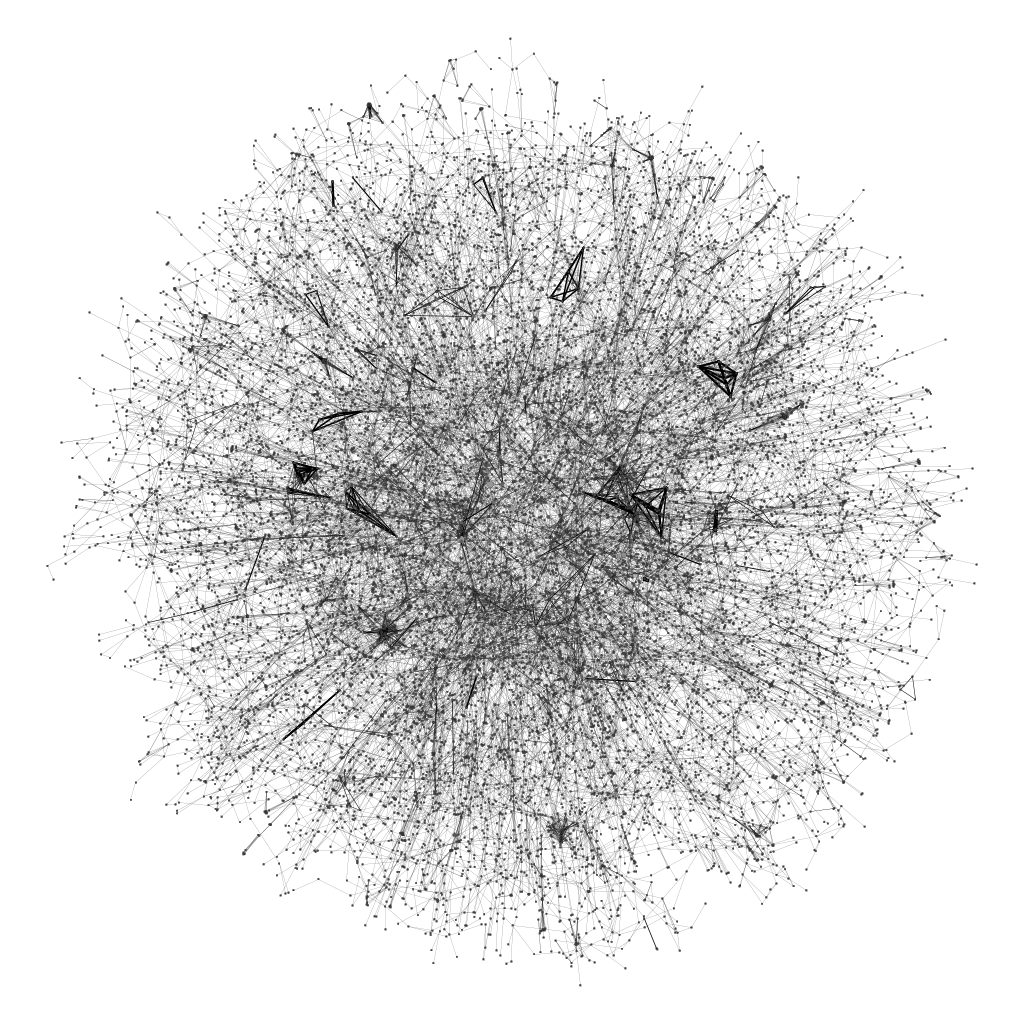
\includegraphics[width=0.5\textwidth]{Giantcomponent.png}
\caption{The sky is the limit.}
\label{fig:giantcomponent}
\end{figure}

\section*{Unnumbered section}
\lipsum[1]

\begin{table}[h]
\def\sym#1{\ifmmode^{#1}\else\(^{#1}\)\fi}
\begin{center}
\caption{The \textit{Two-Independent-Signals} Treatment.\label{table2}}
\vskip 2mm
\setlength\extrarowheight{-5pt}
\begin{tabular}{p{3.5cm} p{4cm}<{\centering}}
\toprule
 & \multicolumn{1}{c}{Posterior Log Odds} \\
\midrule
$\delta$ (Prior Log Odds)&        0.81\sym{***}\\
                         &      (0.05)         \\
\addlinespace
$\beta_{1, T}$           &        0.66\sym{***}\\
                         &      (0.12)         \\
\addlinespace
$\beta_{1, B}$           &        0.81\sym{***}\\
                         &      (0.11)         \\
\addlinespace
$\beta_{2, T}$ (Independent)&        0.60\sym{**} \\
                         &      (0.26)         \\
\addlinespace
$\beta_{2, T}$ (Independent)&        0.39         \\
                         &      (0.26)         \\
\midrule
$P(\beta_{2, T} = \beta_{2, B})$&        0.56         \\
Observations             &         123         \\
\(R^{2}\)                &       0.846         \\
\bottomrule
\end{tabular}
\end{center}
\footnotesize{Notes: *, **, and *** indicate statistical significance at the 0.10, 0.05, and 0.01 levels, respectively. Robust standard errors are in the parentheses.}
\end{table}


\begin{figure}[!h]
\centering
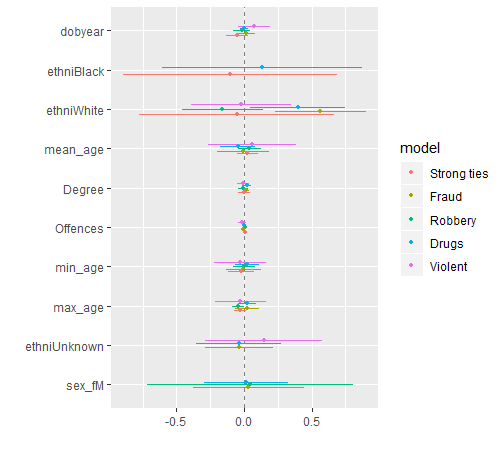
\includegraphics[width=0.8\textwidth]{Reg_highfragment.png}
\caption{The sky is the limit.}
\label{fig:reg_highfragment}
\end{figure}

\section{Second section}

\lipsum[1]

Table \ref{tab:sample_table} is a sample table for illustrative purposes. 

\begin{table}[!h]
\centering
\caption{Sample table.}
\begin{tabular}{cccc}
\toprule
Value 1 & Value 2 & Value 3 & Value 4\\
\midrule
 odd     & odd   & odd & 1.00 \\
 even    & even  & even& 1.00 \\
 odd     & odd   & odd & 1.00 \\
 even    & even  & even& 1.00 \\
\bottomrule
\end{tabular}
\label{tab:sample_table}
\end{table}

\lipsum[1]

\frameboxbegin{Sample frame}
\lipsum[1]
\frameboxend

\newpage

\section{Features commands}

\subsection{Pictures used}

\noindent
Cover picture filename (in titlepage): \texttt{cover}\\
Logo filename (in foot): \texttt{logo}\\
Figure \ref{fig:giantcomponent} (in body): \texttt{giantcomponent} \\
Figure \ref{fig:reg_highfragment} (in body): \texttt{reg\_highfragment}


\subsection{Boxes}

\begin{verbatim}
\fullboxbegin
Content
\fullboxend
\end{verbatim}

\begin{verbatim}
\leftboxbegin
Content
\leftboxend
\end{verbatim}

\begin{verbatim}
\rightboxbegin
Content
\rightboxend
\end{verbatim}

\begin{verbatim}
\frameboxbegin{Frame Title}
Content
\frameboxend
\end{verbatim}


\end{document}          
